% sample.tex
\documentclass[pdf,swa,slideBW,nocolorBG,nototal]{prosper}
%\usepackage{ngerman}
\usepackage{graphicx}
\usepackage{wrapfig, rotating}
\usepackage[T1]{fontenc}

\title{Accumulator}
\subtitle{More Than a Simple Feed-Reader}
\author{Oliver Xylander, Johannes Wollert, Thomas Stoff, Konstantin Haase, Tim Felgentreff}
%\email{\{thomas.stoff, oliver.xylander, konstantin.haase, tim.felgentreff, johannes.wollert\}@student.hpi.uni-potsdam.de}
\institution{
	Softwaretechnik I \\
        Hasso-Plattner-Institut \\
        Universit�t Potsdam\\
	SS 2009 
}
\foot{Accumulator | Softwaretechnik I 2009 | Felgentreff, Haase, Stoff, Wollert, Xylander | \today }

\begin{document}

\maketitle

\overlays{2}{%
\begin{slide}{Introduction}
  \parbox[t]{0.6\textwidth}{%
    \vspace*{1.5cm}
    \hspace*{5cm}
    \begin{rotate}{353}
      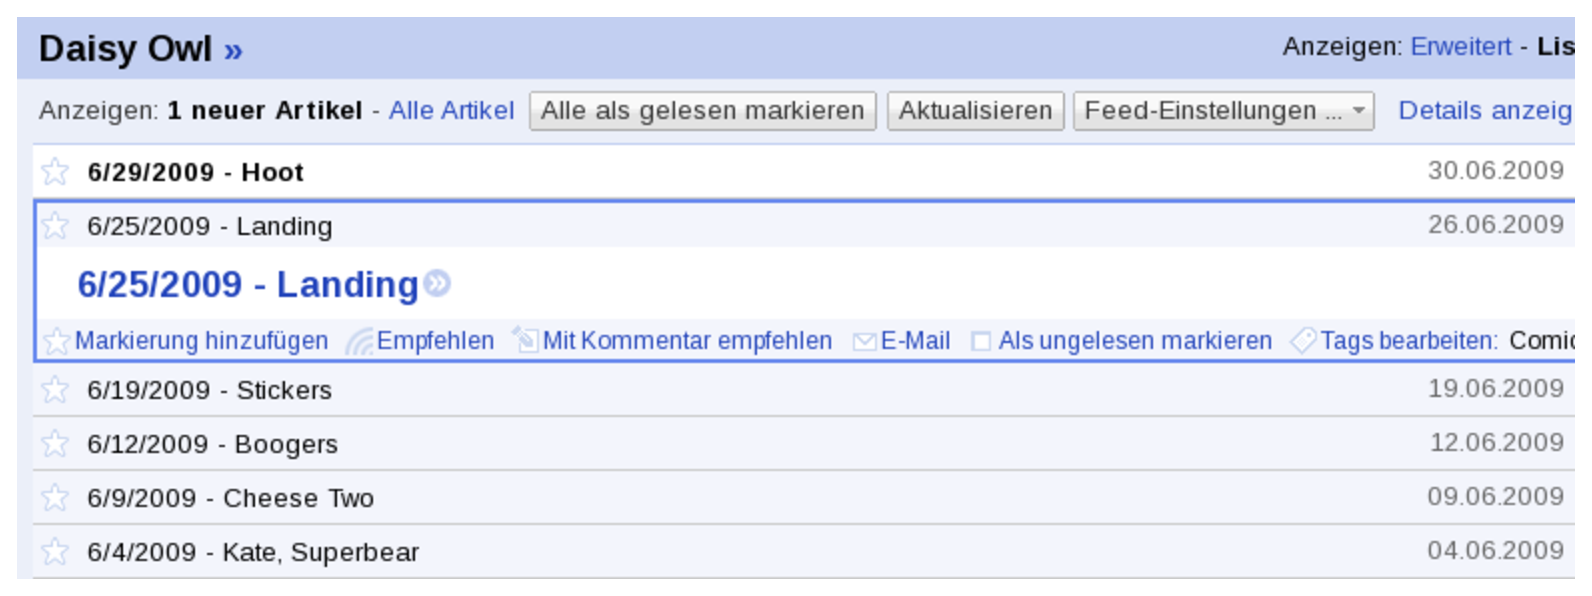
\includegraphics[width=\linewidth]{pics/broken_feed}
    \end{rotate}}
  \begin{minipage}{0.5\textwidth}
    \vspace*{-1.5cm}
    \begin{itemize}
    \item Common Feed-Readers have shortcomings
      \begin{itemize}
      \item RSS-Feeds are often broken
      \item Readers have limited input options
      \item Feeds are only presented as they are
      \end{itemize}
    \end{itemize}
  \end{minipage}
  \fromSlide{2}{%
  \begin{itemize}
    \item The Accumulator is meant to solve some of these
    \begin{itemize}
    \item Filters can fix some feed's problems
    \item We can read more than the common feed formats
    \item Feeds can be tagged and shared
    \end{itemize}
  \end{itemize}}
\end{slide}}

\begin{slide}{Demo}
  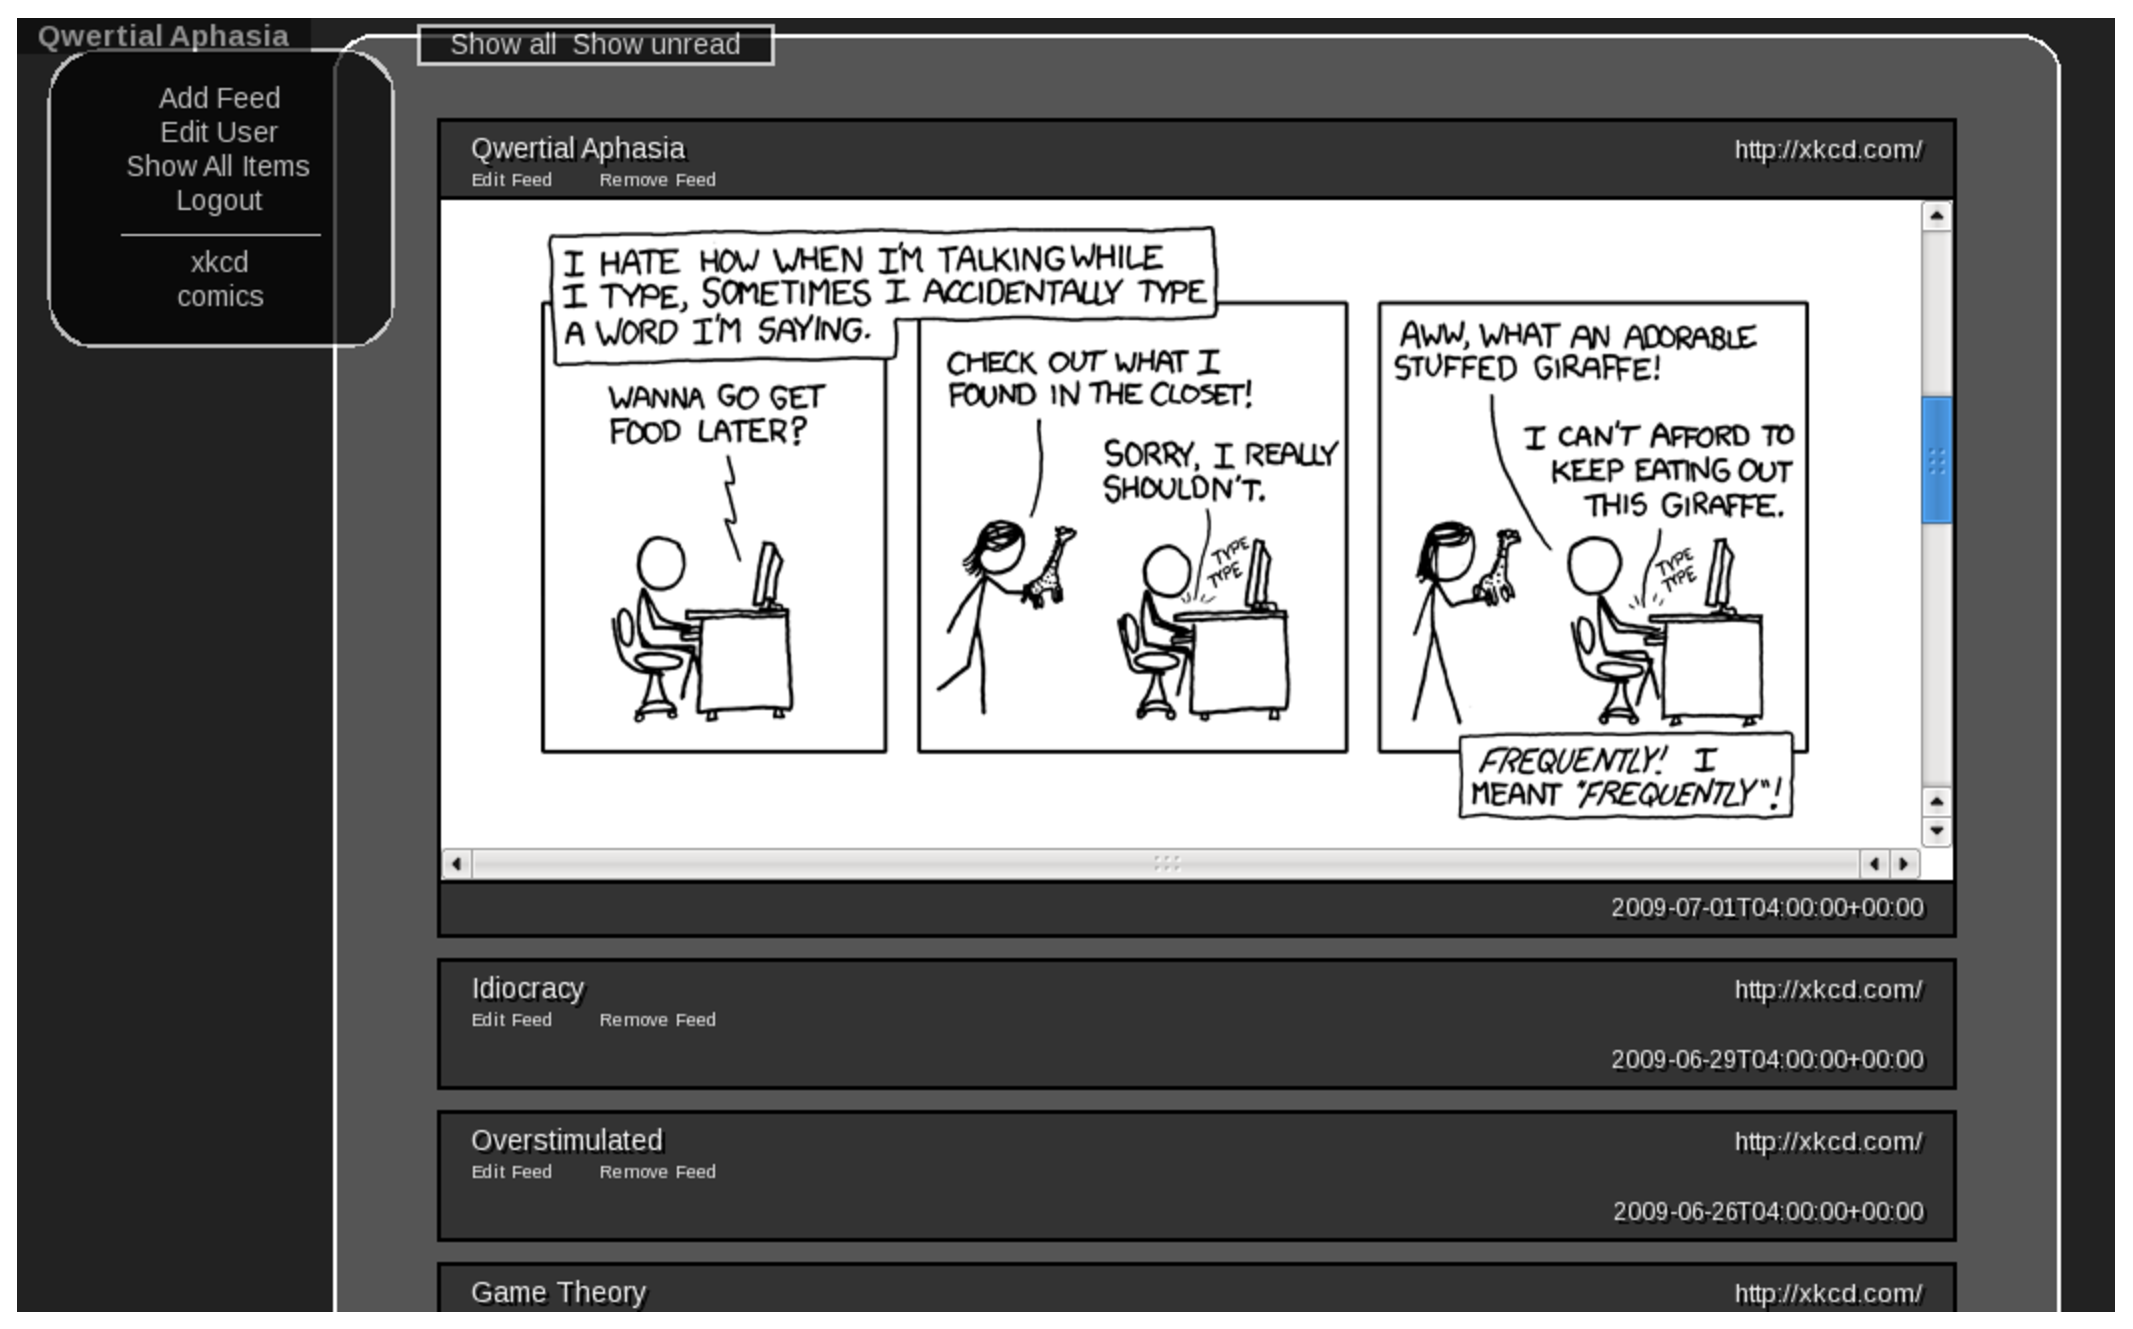
\includegraphics[width=\linewidth]{pics/demo_pic}
\end{slide}

\begin{slide}{Agenda}
  \begin{itemize}
  \item Goals 
  \item Development Process
    \begin{itemize}
      \item Iterations
      \item Xtreme Programming
    \end{itemize}
  \item System Overview
  \item Requirements
  \item Conclusions
  \end{itemize}
  \parbox[t]{0.5\textwidth}{%
    \vspace*{2.5cm}
    \hspace*{7cm}
    \begin{rotate}{12}
      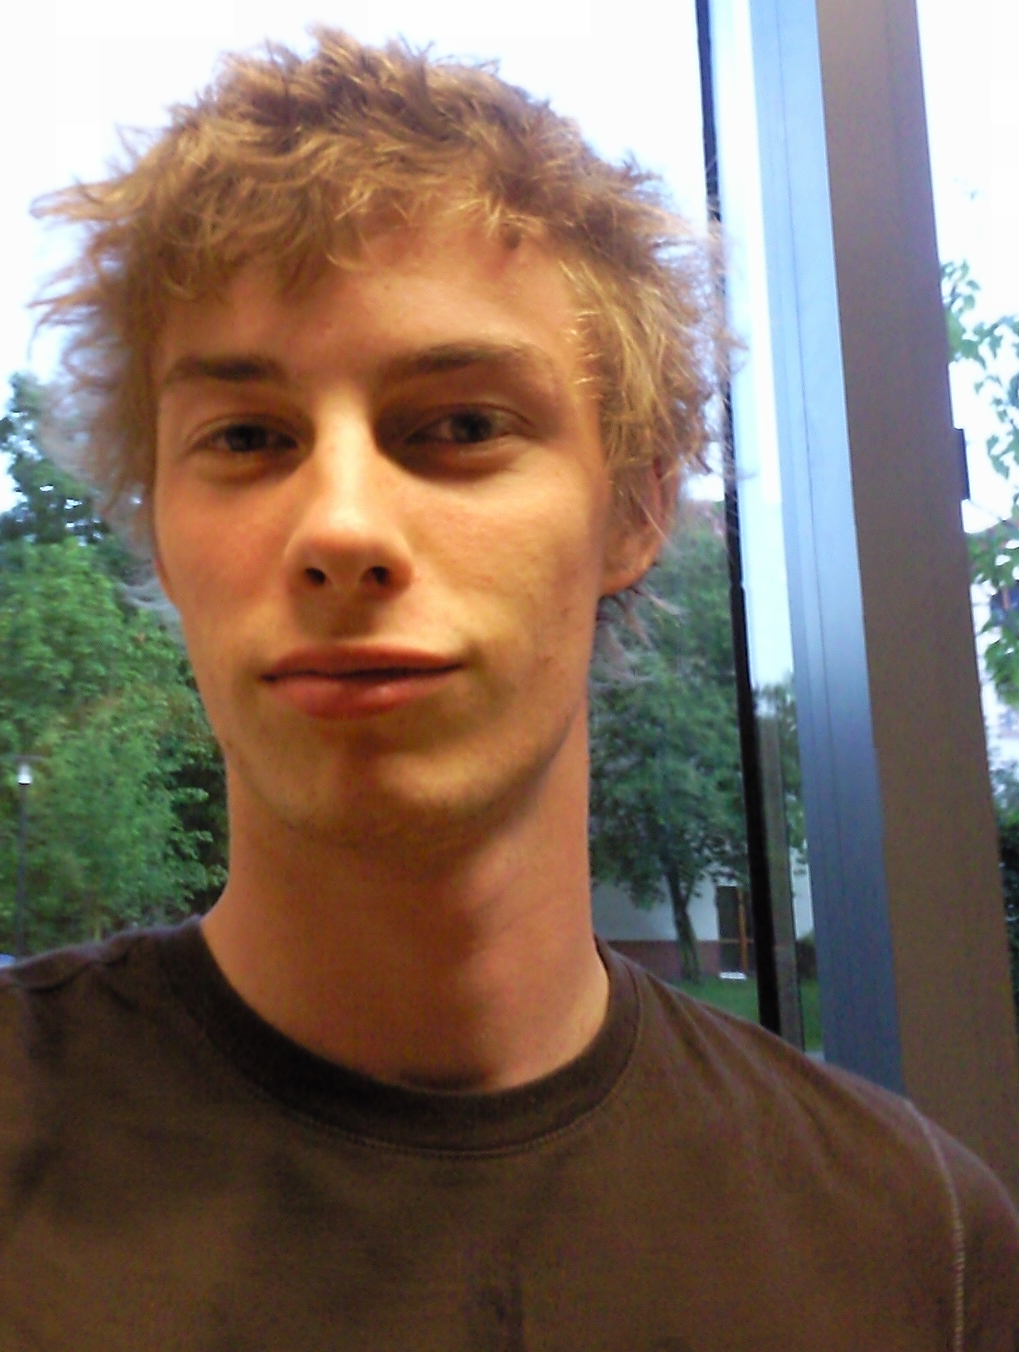
\includegraphics[width=0.9\linewidth]{pics/agenda}
    \end{rotate}}
\end{slide}

\begin{slide}{Goals}
  \begin{itemize}
    \item Read from different sources (RSS, Atom, IMAP, Monticello, Git, \ldots)
    \item Filter sources to ease focus on the things that matter
    \item Be extensible: allow easy integration of new sources and filters
    \item Be open: do not force users into the web-frontend, offer RSS output
  \end{itemize}
  \raggedleft
\includegraphics[width=0.2\linewidth]{pics/git}
\end{slide}

\begin{slide}{Development Process}
  \parbox[t]{0.6\textwidth}{%
    \vspace*{3.5cm}
    \hspace*{5cm}
    \begin{rotate}{353}
      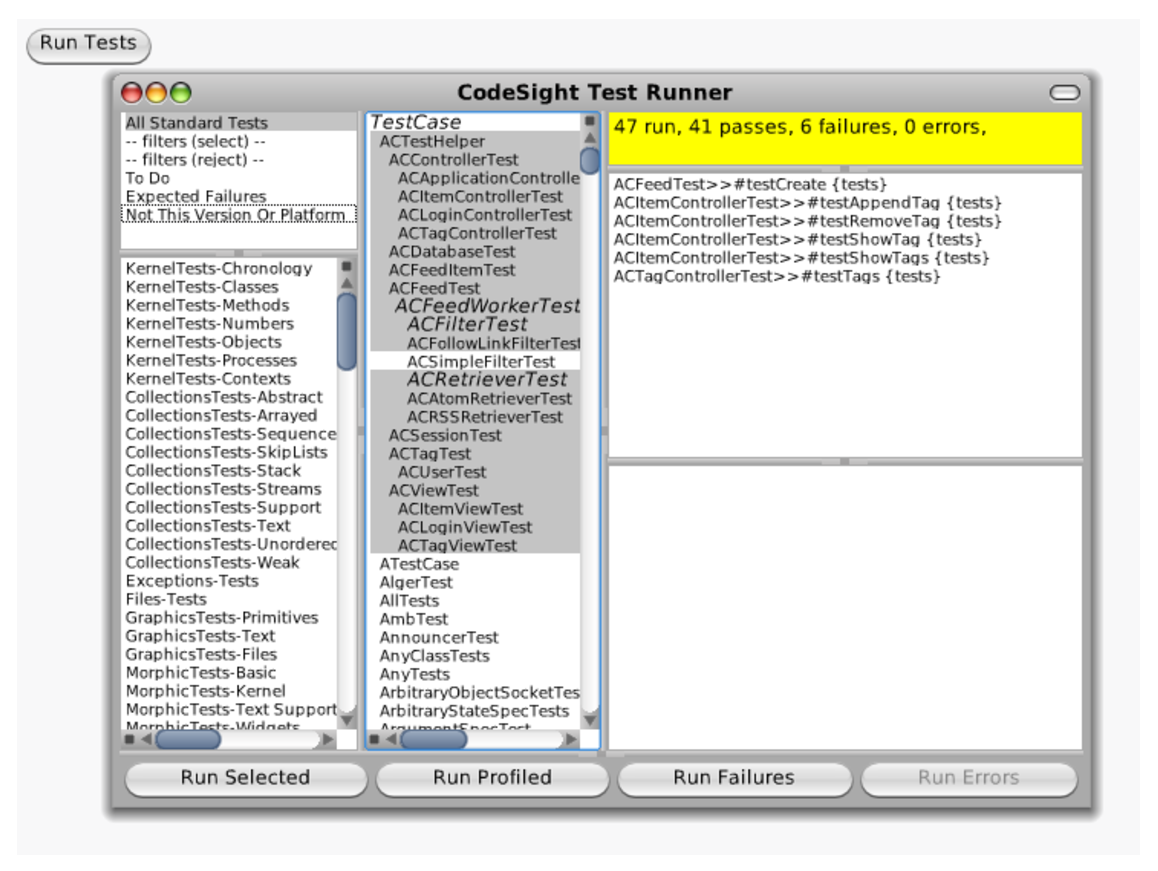
\includegraphics[width=\linewidth]{pics/tests}
    \end{rotate}}
  \vspace*{-3.5cm}
  \begin{itemize}
    \item Xtreme Programming
      \begin{itemize}
	\item {\tiny Planning game}
	\item {\LARGE Pair programming}
	\item {\large Small releases}
	\item {\footnotesize On-site customer}
	\item {\Large Test-Driven-Development}
	\item {\LARGE Refactoring}
	\item {\tiny Coding Standards}
	\item {\normalsize Simple Design, Metaphor}
      \end{itemize}
  \end{itemize}
\end{slide}

\begin{slide}{Iterations and Milestones}
  \includegraphics[width=\linewidth]{pics/drawing}
\end{slide}

\begin{slide}{Development Process (contd.)}
  \begin{itemize}
    \item Pair Programming
      \begin{itemize}
	\item Working in two's or three's
	\item Two or three teams working alongside on different parts of the system
	\item Working in one room, each team on two or more monitors
	\item Development by smoke-break
      \end{itemize}
  \end{itemize}
\end{slide}

\begin{slide}{Development Process (contd.)}
  \begin{minipage}{0.5\textwidth}
    \begin{itemize}
      \item Planning Game and Small Releases
	\begin{itemize}
	  \item Once every week
	  \item Bring everyone up-to-date with the latest changes
	  \item Discussion of last-weeks changes
	  \item Assignment of user stories to new pairs
	\end{itemize}
    \end{itemize}
  \end{minipage}
  \parbox[t]{0.5\textwidth}{%
    \vspace*{2.5cm}
    \hspace*{7cm}
    \begin{rotate}{8}
      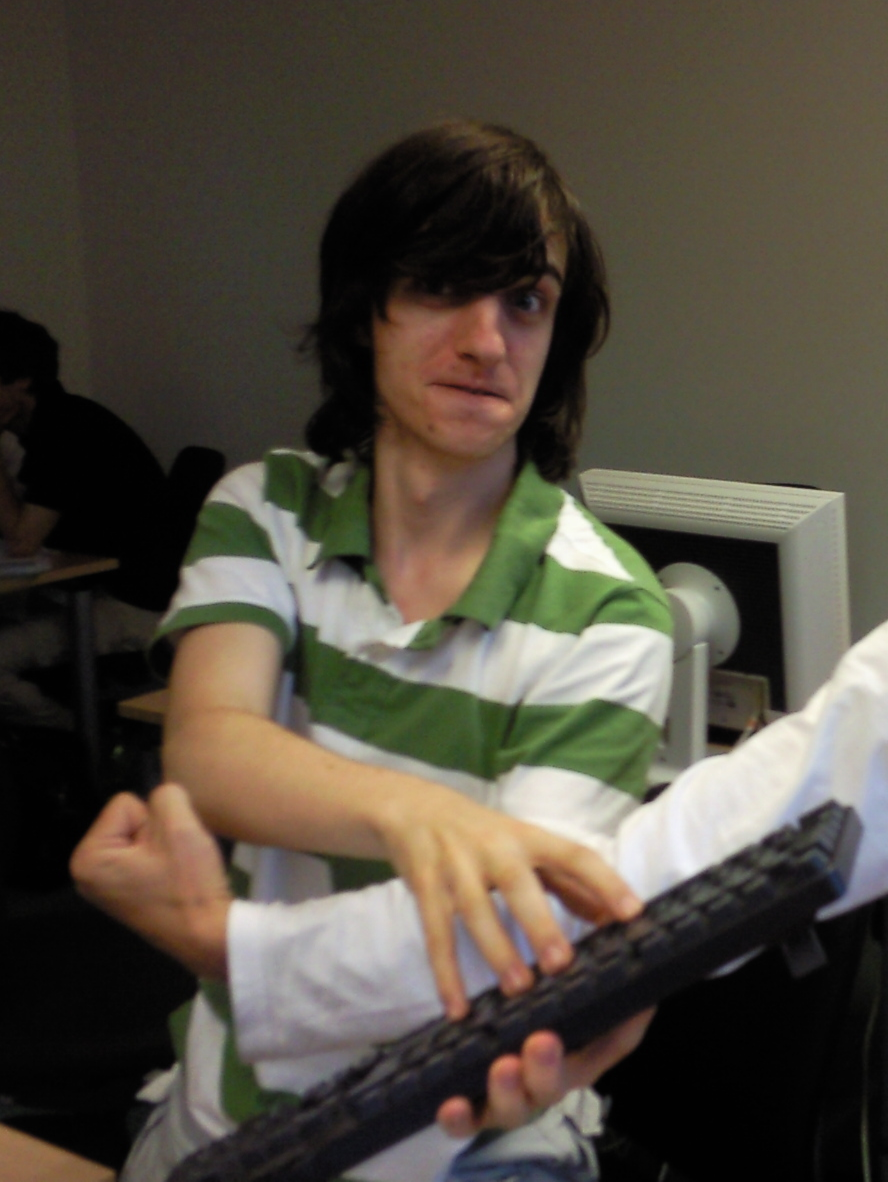
\includegraphics[width=0.9\linewidth]{pics/standup}
    \end{rotate}}
\end{slide}

\begin{slide}{Development Process (contd.)}
  \begin{itemize}
    \item Test-Driven-Development
      \begin{itemize}
	\item The first hint of an API gets a (failing) test-case
	\item Test cases are in flux - they are examples as much as tests
	\item Methods not covered by tests should not be refactored
	\item Test cases that belong to a single interface are completed 
	  in one swift session
	\item SUnit was extended with \\more testing capabilities \\(Mutations, Call-Counts)
      \end{itemize}
  \end{itemize}
  \parbox[t]{0.6\textwidth}{%
    \vspace*{2.5cm}
    \hspace*{5cm}
    \begin{rotate}{353}
      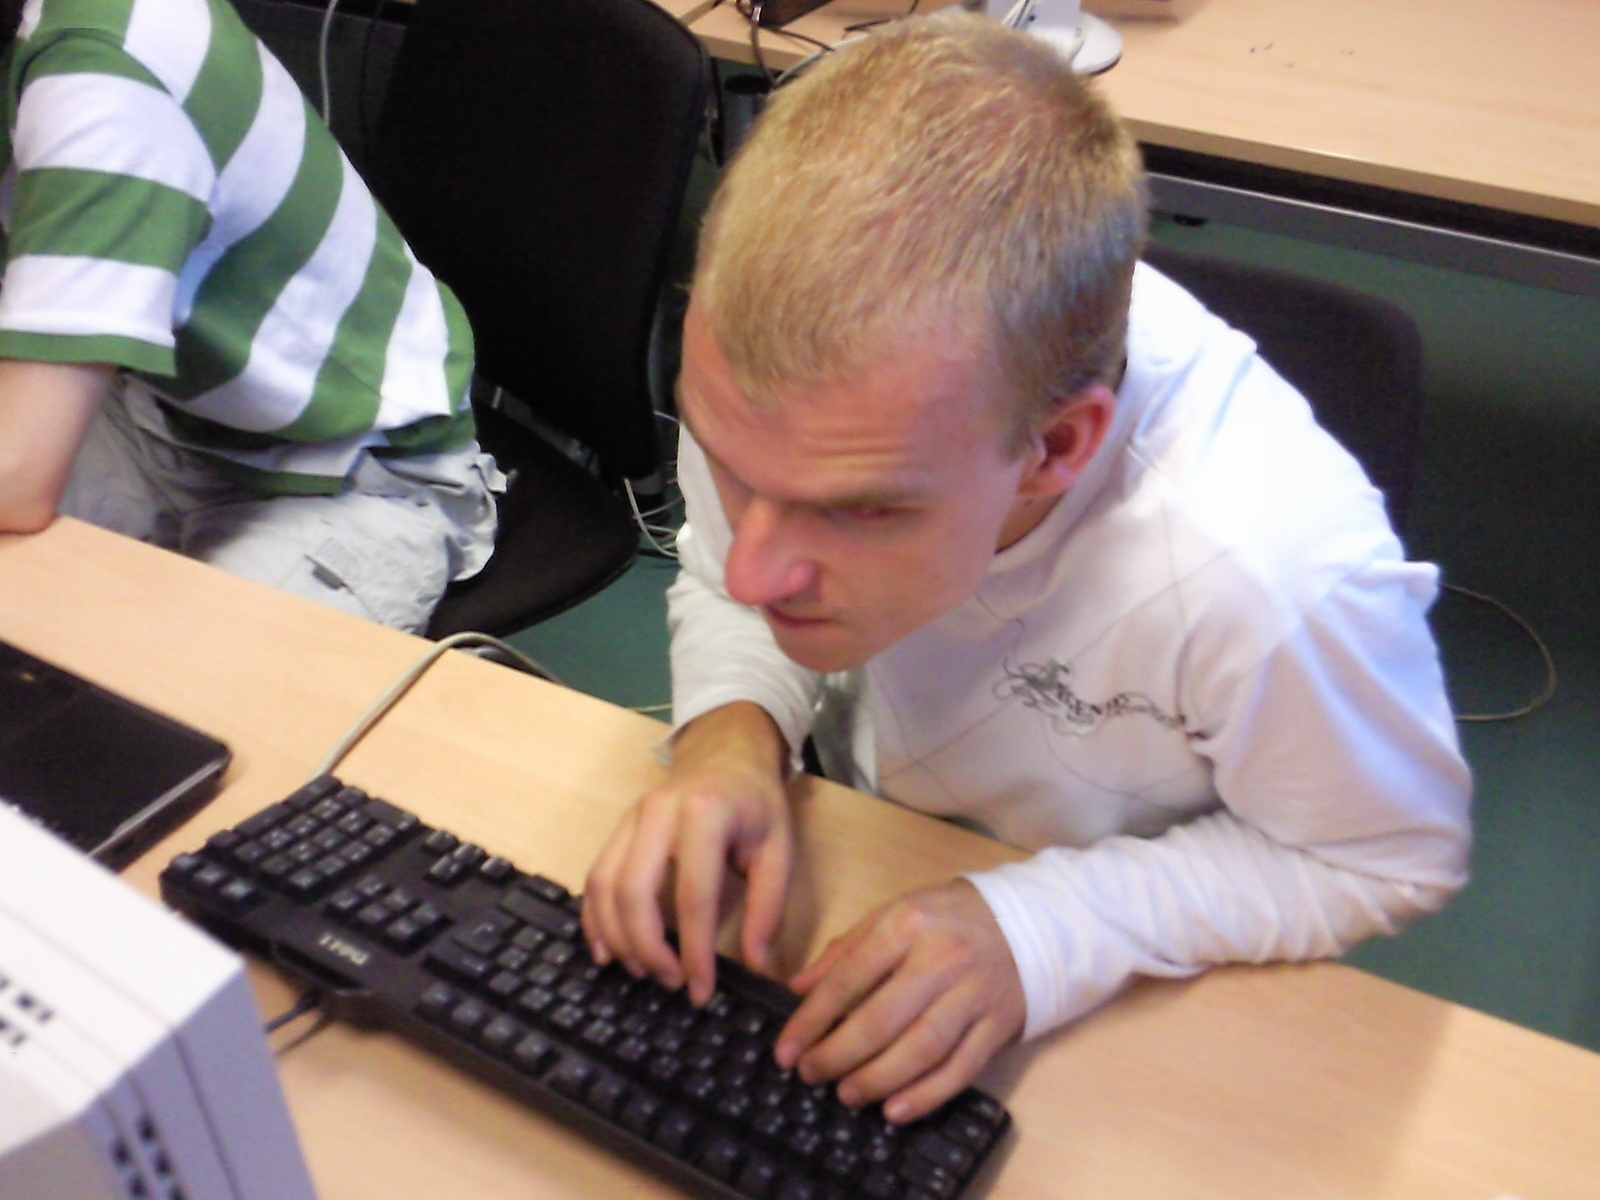
\includegraphics[width=\linewidth]{pics/Foto0326}
    \end{rotate}}
\end{slide}

\begin{slide}{Development Process (contd.)}
  \begin{itemize}
    \item Coding Standards and Refactoring
      \begin{itemize}
	\item Always have a running version
	\item After each change: run the test suite
	\item Each commit should (within reason) be usable
	\item Non-local commits should always add a feature or fix a bug
	\item Breaking commits should be local
      \end{itemize}
  \end{itemize}
\end{slide}

\begin{slide}{System Overview}
  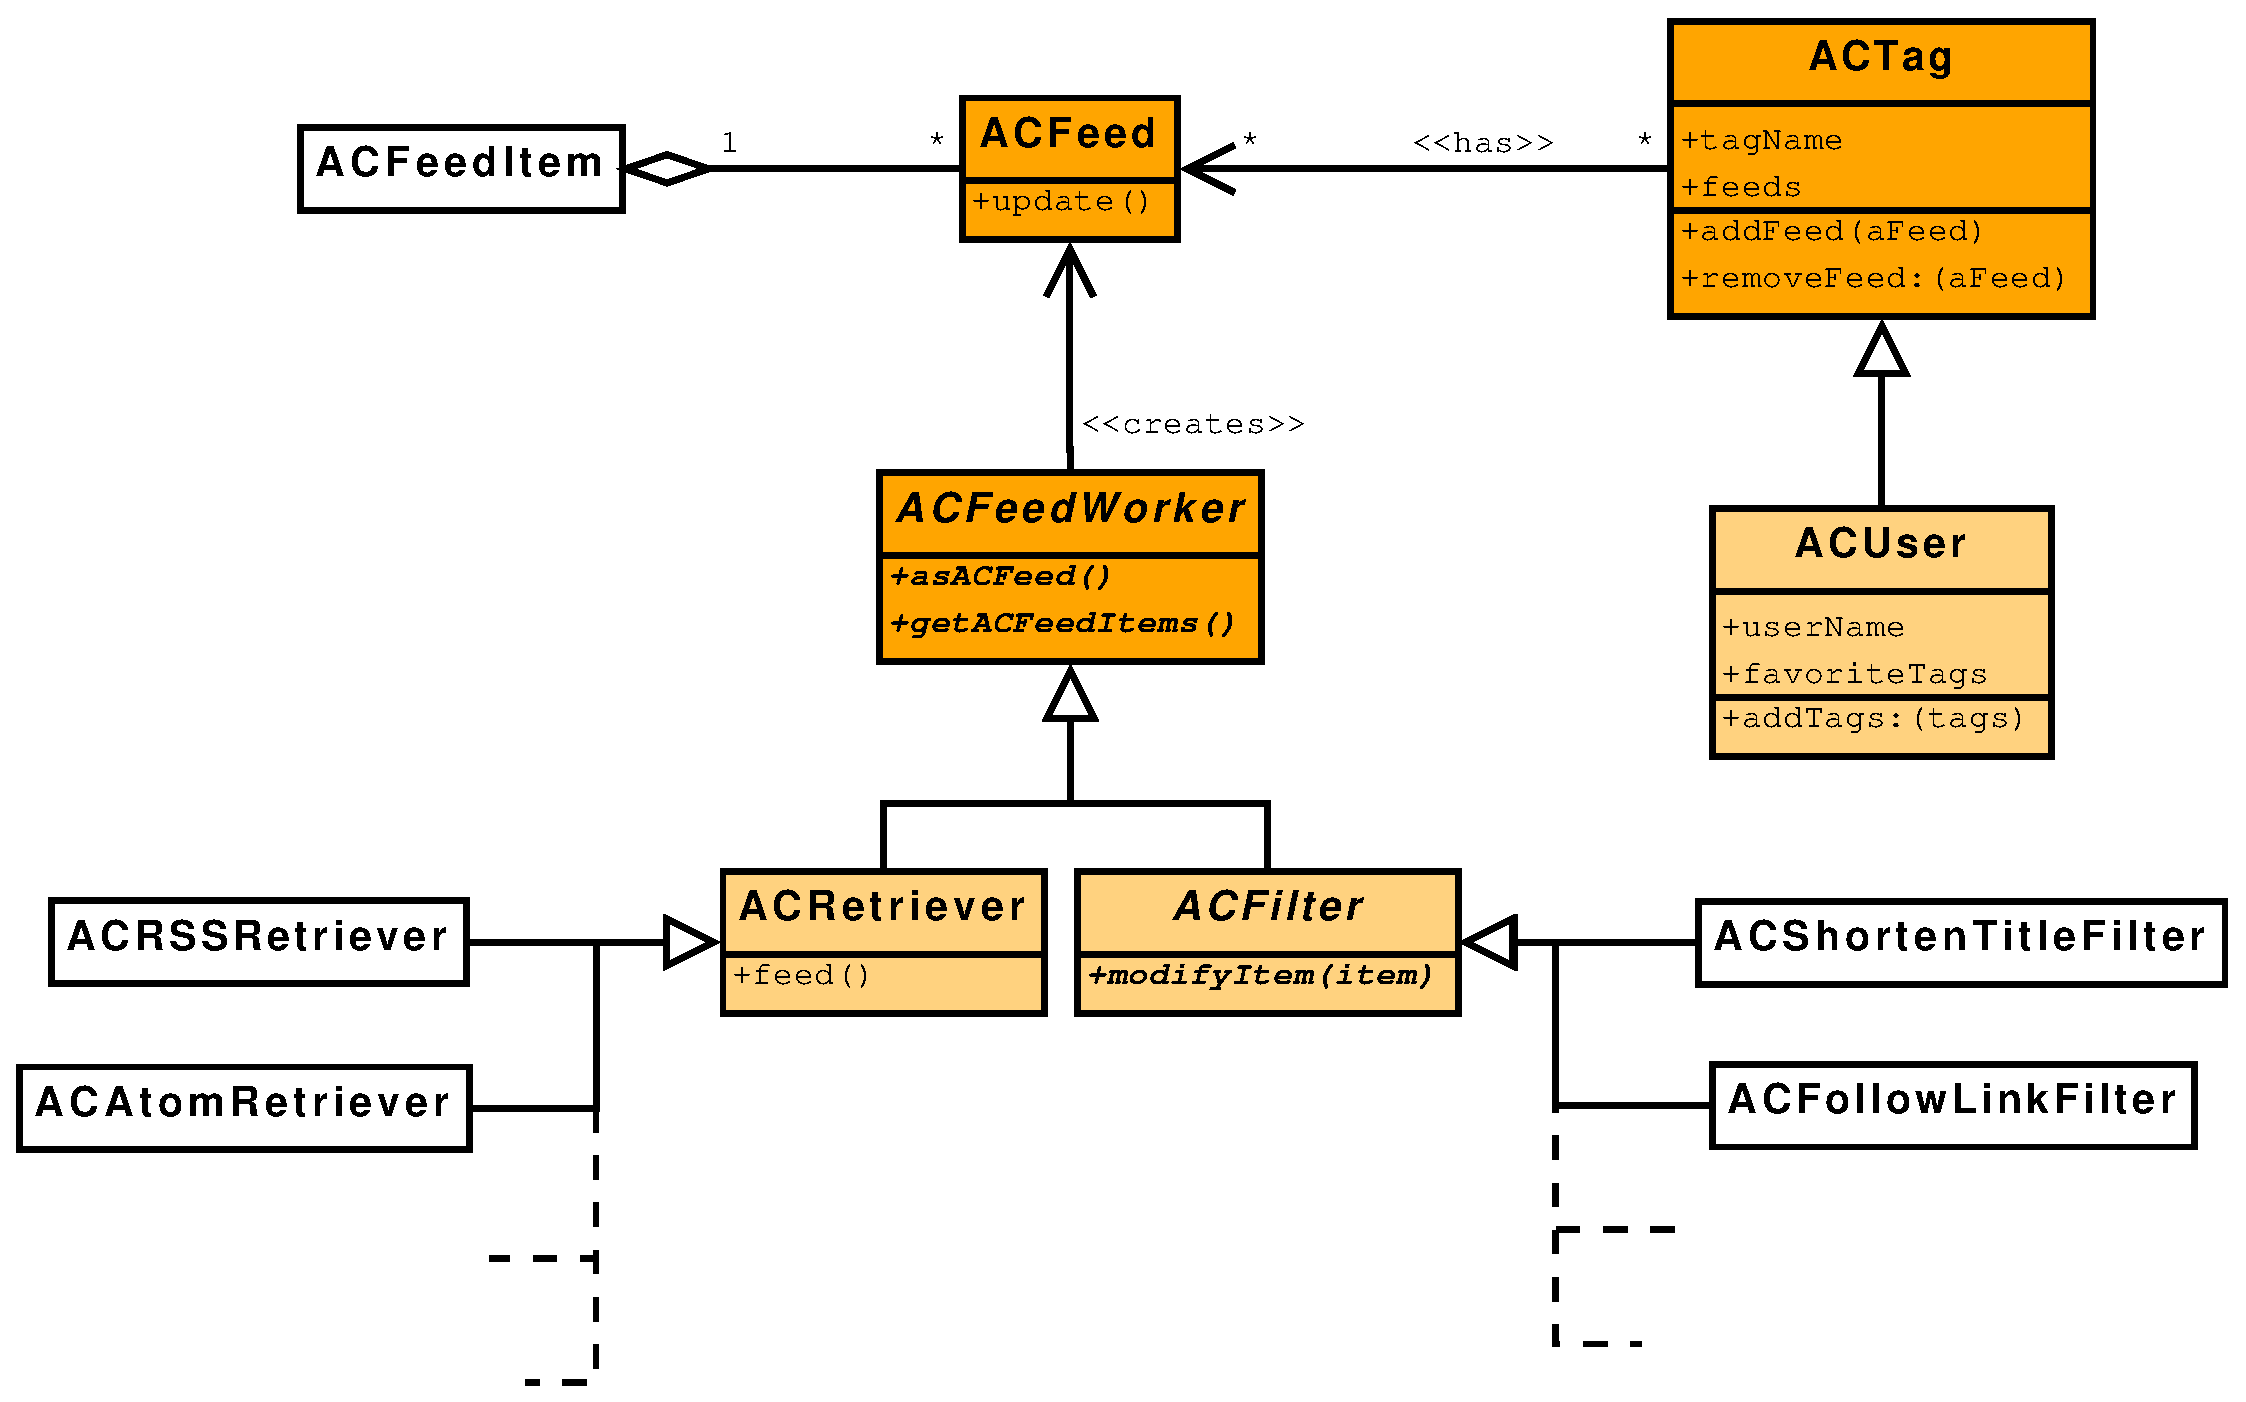
\includegraphics[width=\linewidth]{pics/system}
\end{slide}
\begin{slide}{Working the Code}
  \begin{itemize}
    \item Convention over Configuration
      \begin{itemize}
	\item MVC Pattern
	\item Convenience method aliases	
      \end{itemize}
    \item Magritte 
    \item Testing with mutations
  \end{itemize}
\end{slide}

\overlays{2}{%
\begin{slide}{Requirement Tracing: Filters}
  \begin{greenbox}
    \textcolor{white}{
    ``Carl-Maria is pretty annoyed with Fefe's RSS-Feed. He would like
    to have it's title properly displayed in the content area, and 
    at the same time shorten the title to only show the beginning of 
    the first line. To do this, he adds two simple filters to the feed''}
  \end{greenbox}
  \fromSlide{2}{%
  \begin{itemize}
    \item[] ~\\
    \begin{itemize}
      \item Offer a set of simple, well-defined filters
      \item Allow chaining of those filters to offer powerful filtering
      \item Create   test-cases as contract for the I/O requirements
      \item Write the filter functionality and make it pass the tests
      \item Expose the filter through the frontend
    \end{itemize}
  \end{itemize}}
\end{slide}}

\overlays{2}{%
\begin{slide}{Requirement Tracing: Server Resources}
  \begin{greenbox}
    \textcolor{white}{
    ``The client would like to deploy the system on his server. 
    However, due to limited bandwidth and filesystem space, he cannot 
    afford each feed for each user to be downloaded separately''}
  \end{greenbox}
  \fromSlide{2}{%
  \begin{itemize}
    \item[] ~\\
    \begin{itemize}
      \item Make sure each feed in the system is unique, so saving and 
	downloading per feed is only done once
      \item Users share the same feeds
      \item Per-user feeds are realized by adding feeds to the user's tags
    \end{itemize}
  \end{itemize}}
\end{slide}}

\overlays{2}{%
\begin{slide}{Requirement Tracing: Tagging}
  \begin{greenbox}
    \textcolor{white}{
    ``Johannes feels, directory hierarchies do not account for 
    the diversity of information available in feeds. He'd much 
    rather assign topics to feeds and be able to select feeds by
    topic. If at it, he would also love to be able to read what other 
    people read on this topic''}
  \end{greenbox}
  \fromSlide{2}{%
  \begin{itemize}
    \item[] ~\\
    \begin{itemize}
      \item Use tagging instead of directories
      \item Feeds can have arbitrary tags - by selecting 
	tags, the user gets a selection of feeds which belong 
	to all selected tags
      \item A user is just a tag himself - when removing the user 
	from the tag selections, tags from other users can be shown
    \end{itemize}
  \end{itemize}}
\end{slide}}

\begin{slide}{Looking back\ldots}
  What we think we did well\ldots
  \begin{itemize}
    \item Steady workflow
    \item Balance between ``Get that feature in'' and ``Code cleanup''
    \item Keeping the test-suite ahead of the code
    \item Keeping the system in working order
  \end{itemize}
\end{slide}

\begin{slide}{\ldots and looking ahead}
  What we would like to do differently\ldots
  \begin{itemize}
    \item Spend more time on bug-fixing
    \item Better iteration planning (or at least some planning at all)
    \item Keeping the test-suite ahead of the code
    \item Use a better version-control-system (MC2, Git, \ldots)
  \end{itemize}
\end{slide}

\overlays{2}{%
\begin{slide}{On XPForums and SqueakSave}
  \begin{itemstep}
    \item XPForums
      \begin{itemize}
	\item User stories were helpful
	\item Associations with code could have been better
	\item VNC never worked for us
	\item Never used code markup, rather discussed that in the meeting
      \end{itemize}
    \item SqueakSave
      \begin{itemize}
	\item A great step up from configuring GLORP
	\item Nice concepts (Object>>save, Connection pools)
	\item Some loose ends and not too helpful error messages \\
	  $\Rightarrow$ {\tt Database reset} was a frequent ``Do it''
      \end{itemize}
  \end{itemstep}
\end{slide}
}

\begin{slide}{Sources}
  \nocite{*}
  \bibliographystyle{splncs}
  {\small \bibliography{swt.bib}}
\end{slide}

\end{document}
